\documentclass[a4paper]{article}
\usepackage{graphicx} 
\usepackage{amsmath}

\usepackage{geometry}
\usepackage{pdfpages}
\usepackage{url}
\usepackage{parskip}
\usepackage{listings}
\geometry{
	tmargin=15mm,
	lmargin=15mm,
	rmargin=15mm,
	bmargin=15mm
}
\usepackage{cite}

\hyphenation{op-tical net-works semi-conduc-tor}
\usepackage{stfloats}


\title{MATH3208 - Optimization Coursework}
\author{Azhagesh
	Azhagesh, Ashwinkrishna\\
	\texttt{aa9g22@soton.ac.uk, University of Southampton}
}
\begin{document}
    \maketitle





    The problem of finding the optimal orientation and position of irregularly shaped objects in a finite area, is inherently NP-complete \cite{Nonregular} if you approach this with infinite orientations and positions possible, in a finite ability 2d space where the shape of the area can change ie rectangle, triangular 2d plane etc. Even if you want to pack irregular objects in a rectangle 2d space, in the most efficient manner, which reduces complexity as 1. it is not an arbitrary shape but a rectangle, and, which is fixed, the problem is still combinatorial and NP-hard, and more famously we can redefine this beyond the simple four animal puzzle.\\

    I see this in a more general sense, of wanting to fit four irregular shapes inside a rectangular container and taking into account the various possible orientations and positions these shapes can take. This is a famous problem, as it can be classified as a nesting problem \cite{irregular}. Now even if we were to remove the rotational constraint or orientation, this is still an NP-hard problem. Hence, an algorithm that can find the optimal or close to optimal solution with an irregular shape in a rectangular plane in the most efficient manner possible isn't likely to be polynomial time complexity.\\

    Now the approach takes in \cite{bismark} of using the inclusion-exclusion principle and using heuristics by measuring the cutouts, manually trying out all 48 possible permutations and then generating a dataset of the two shapes in the allowed orientations, and then finally using a program to effectively calculate the minimum amount of width needed, such that these shapes fit inside the minimum rectangle possible. This is slightly different from the original paper as the puzzle \cite{mongolia} as that had a hexagonal box where you had to place the pieces, instead of a rectangle.\\

    One of the problems with utilising the inclusion-exclusion and taking this particular approach is that you have to manually measure the distance, and make a cutout of the irregular shapes, which have scaling errors. Then use these cutouts to try possible orientations and combinations, manually checking that the shapes do not overlap when you do measure the least width possible. Therefore this process is very time-consuming and isn't feasible for a larger amount of shapes. One potential way to mitigate this is, as seen in the first paper \cite{mongolia}, to model the shapes as a circle which reduces, the measurements needed, but this is also very inefficient and leaves a lot of gap between the shapes, isn't close to being optimal.\\

    
    So one way to approach this problem is to in a similar fashion to paper 1 \cite{mongolia}, model the shapes roughly, as a rectangular shape. This simplifies the algorithm needed to fit this in the smallest rectangle possible. \\

    So the way I went about my initial solution here, is I used Golang as the language, due to its fast execution speed in comparison to Python, and compile times. I started off by modelling what I was going to do and thought about various edge cases and issues that might occur. So firstly I made a struct type in Golang, that defines a rectangle. This struct has two variables, which are height and width. Then utilising this I make a slice of this custom type, reading the measurements from the pdf, in real life this can be automated with computer vision techniques and openCV, this is what shipping containers do \cite{packing}, this information of the height and width was then written in manually, but it can be automated with the methods suggested before.\\

    Next, there was the issue of possible permutations of the rectangular shapes, which can either be 0 or 90 degrees, intuitively you can understand due to the symmetrical properties of rectangles it isn't worth trying to do 180 or 360 degrees, also due to our problem of trying to fit the shapes into the smallest space possible, we can conclude that it's best if the faces of the rectangle are parallel so as to minimise the wastage of space. Given we have four shapes we need to consider all possibilities, so 2 raised to 4, is 16 possibilities, which is lower than the 48 considered in this paper \cite{bismark}, (but yes I understand this is worse off long term, as you can approach it dynamically with inclusion-exclusion to get better faster results, given you remeasure for every prime.). \\

    So I wrote a combinatorics function that generates all possible combinations, either 0 or 90 degrees in 4 positions. \\


    \[
\begin{bmatrix}
0 & 0 & 0 & 0 \\
90 & 0 & 0 & 0 \\
0 & 90 & 0 & 0 \\
90 & 90 & 0 & 0 \\
0 & 0 & 90 & 0 \\
90 & 0 & 90 & 0 \\
0 & 90 & 90 & 0 \\
90 & 90 & 90 & 0 \\
0 & 0 & 0 & 90 \\
90 & 0 & 0 & 90 \\
0 & 90 & 0 & 90 \\
90 & 90 & 0 & 90 \\
0 & 0 & 90 & 90 \\
90 & 0 & 90 & 90 \\
0 & 90 & 90 & 90 \\
90 & 90 & 90 & 90
\end{bmatrix}
\]



Then for the sake of simplicity, I use a loop to iterate through these possibilities, and if the angle is 0, I add the original width of the shape, if it is rotated, so 90, I then add the original length of the rectangular shape to the width, and at the end I have a list of possibilities, all the total widths and the max height, of the rectangular prism in each case, which is printed at the end. Then taking the minimum of the value, of the width, I print that out to the screen along with the corresponding height of that rectangular prism, along with the area.\\

   Now the time complexity of this approach is 2\^n, and given this problem is NP-complete it is unlikely for me to come up with a polynomial time solution for this problem. I wish I could though. Anyway, this approach can be improved and this is a basic proof of concept. Shipping containers and companies face the problem of efficiently packing irregular sometimes even curved objects into a 3d space, which is a much harder problem. One way we can improve this is through is by thinking of larger shapes as smaller rectangles and then adding rules so that the rectangle in question can't rotate and is fixed to the larger rectangle, then when you split up a shape into small enough rectangles you get a pixelated image. So this approach might be a quick and simple way of doing this in OpenCV, however, it isn't anywhere close to being as efficient as it can be.\\


    So far I've avoided using external libraries, but now I'm going to switch to Python and approach this problem as an irregular bin packing problem in Python, mainly because it'd be faster to code this in using libraries than manually having to reinvent the wheel in Golang. (However, I do recommend Golang, C, or C++ for a larger amount of shapes). \\

    So to start off I made a new virtual environment in Python and installed some libraries like matplotlib to visualise what was going on, then I used shapely to build on top of this library rather than implement this from scratch. To avoid having to rewrite the polygon logic from scratch, and implement things like collision detection, areas, bounds etc, I used Shapely's geometry methods and imported into Polygon. This is used to model the irregular objects inputted into the algorithm.\\

    To address the rotations, I imported the rotation methods, and this allows me to rotate a shape around the centroid, while the translation methods move the shape along the x and y-axis. Finally, to help visualise what was happening I used matplotlib to plot the final positions the shapes ended up in.\\

    Next, I created a polygon function that takes in the points, in the form of x y, coordinates as tuples and then returns the shapely polygon object, which we can then apply various operations like rotation/translation on. The next function I made allows me to do this, by passing in the angle I can rotate the polygon object, while it maintains its spacial alignment between the points. We now need a method to move the polygon so we can place it in an orientation and position in a 2d plane, to avoid collisions/overlap between objects, which is what the move polygon function handles. \\


    I've taken a greedy approach to this problem so the greedy place algorithm, takes in the shapes, the container dimensions, and the angles you want to try out, to rotate the shapes, I made the angles a discrete set to try rather than trying every possibility. I moved it in increments of 5 units across at the beginning for the sake of speed, then I improved it so that it moves in smaller increments of 0.1, and rotates if needed to find the best possible fit. The images below will show the improvements made by this approach.\\

    Finally, to visualise the shapes and the plane, I use the plot shapes function to plot out what happened with matplotlib. \\

    In order to model the shapes I took screenshots of the images in \cite{bismark}, then I used a graphical tool called vector to decrease the opacity of the images that have been pasted in, and then traced out the path of the object with the grid overlay, allowing me to count the position of the vertices I drew. Then this was translated into the coordinates of the polygon.\\



    \begin{center}
    \begin{minipage}{0.48\textwidth}
        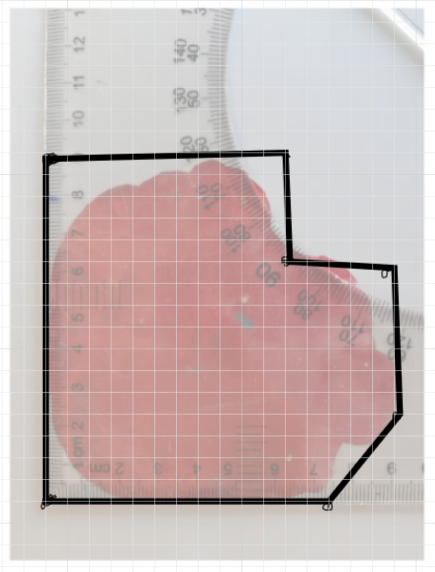
\includegraphics[width=6cm]{Image_1_plot}
    \end{minipage}
    \hfill
    \begin{minipage}{0.48\textwidth}
        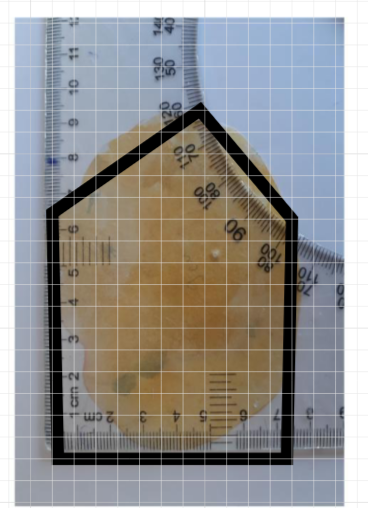
\includegraphics[width=6cm]{Image_2_plot}
    \end{minipage}

    \vspace{0.5cm}

    \begin{minipage}{0.48\textwidth}
        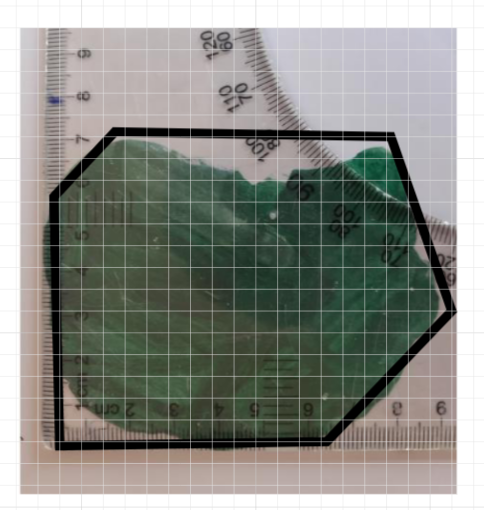
\includegraphics[width=6cm]{Image_3_plot}
    \end{minipage}
    \hfill
    \begin{minipage}{0.48\textwidth}
        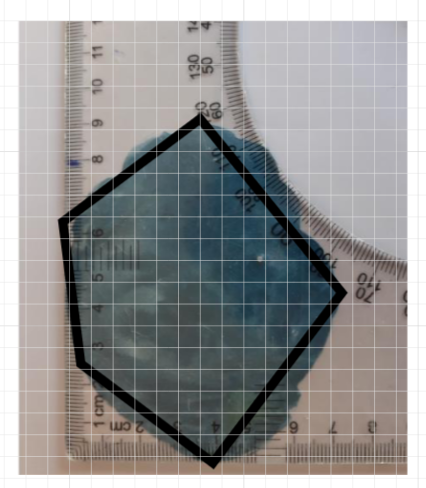
\includegraphics[width=6cm]{Image_4_plot}
    \end{minipage}
\end{center}


\section{Results: }

\begin{figure}[h]
    \centering
    \begin{minipage}[b]{0.45\textwidth}
        \centering
        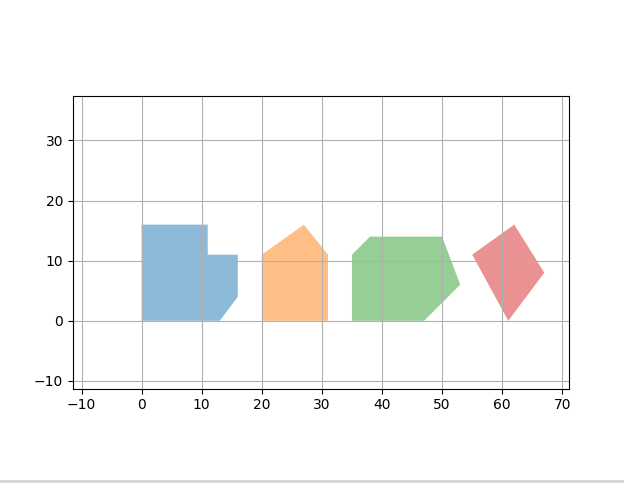
\includegraphics[width=7cm]{Image_5}
        \caption{Original with 5-unit increments}
        \label{fig:original}
    \end{minipage}
    \hfill
    \begin{minipage}[b]{0.45\textwidth}
        \centering
        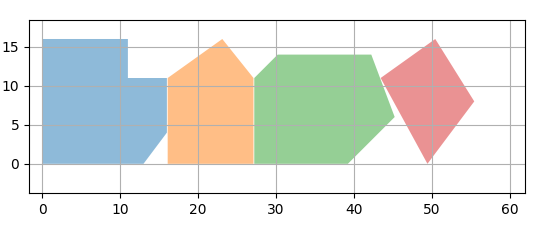
\includegraphics[width=7cm]{Image_7}
        \caption{Improved version with 0.1-unit increments}
        \label{fig:improved}
    \end{minipage}
    \caption{Comparison between the original and improved versions}
    \label{fig:comparison}
\end{figure}

\section{Future suggestions and limitations of the model: }

So while taking a greedy approach is one manner to approach this problem there are some limitations with the methods I have used. One of the main limitations of this approach is that I did not use computer vision techniques, so I had to manually plot the points of the polygon into the algorithm, but the current codebase gives a good foundation for future works, where you can easily integrate some sort of openCV model so that this part of the algorithm can be automated. This will significantly save time, another aspect in which this program can be improved is that we can extend the already existing method, or use other heuristics and approaches such as rectangular packing, and sweeping pieces until you find a position that works with multiple orientations and positions, and sweeping with gravity so the pieces are in the lowest position possible without collisions etc. All of these other approaches are interesting and possibly one might be more efficient than the other depending on the shapes involved so this is an extension that can be done to improve the codebase. One more thing is that my algorithm is efficient if the increment is small but this means the program heck every small increment, and the way I have implemented this part of the code can be improved quite easily, by skilling to the edges of the shapes given certain conditions are met. \\ 

There is also a neural network approach you can use, by using AI to train a model that focuses on placing objects in a container. Overall I think given the timeframe we had to work, and the efficiency needed for four shapes my approach fits this problem quite well. I will paste some screenshots of the code in the appendix.\\ 






 \newpage    

\section{Appendix: }

\subsection{Code: }


\begin{verbatim}

from shapely.geometry import Polygon
from shapely.affinity import rotate, translate
import matplotlib.pyplot as plt
import numpy as np 

def create_polygon(points):
    return Polygon(points)

def rotate_polygon(polygon, angle):
    return rotate(polygon, angle, origin='centroid')

def move_polygon(polygon, x_offset, y_offset):
    return translate(polygon, xoff=x_offset, yoff=y_offset)


def greedy_place(shapes, container_width, container_height, rotation_angles=[0, 90, 180, 270]):
    placed_shapes = []

    for shape in shapes:
        placed = False
        for angle in rotation_angles:
            rotated = rotate_polygon(shape, angle)
            minx, miny, maxx, maxy = rotated.bounds
            shape_width = maxx - minx
            shape_height = maxy - miny

            # Sweep across container area
            for y in np.arange(0, int(container_height - shape_height), 0.1):
                for x in np.arange(0, int(container_width - shape_width), 0.1):
                    candidate = move_polygon(rotated, x - minx, y - miny)

                    # Check collision with all placed shapes
                    if all(not candidate.intersects(p) for p in placed_shapes):
                        placed_shapes.append(candidate)
                        placed = True
                        break
                if placed:
                    break
            if placed:
                break

        if not placed:
            print("Shape could not be placed.")
    
    return placed_shapes


def plot_shapes(shapes, container_width, container_height):
    fig, ax = plt.subplots()
    for shape in shapes:
        x, y = shape.exterior.xy
        ax.fill(x, y, alpha=0.5)

    ax.set_xlim(0, container_width)
    ax.set_ylim(0, container_height)
    ax.set_aspect('equal')
    plt.grid(True)
    plt.show()



# Define some sample shapes
shape1 = create_polygon([(0,0), (13,0), (16,4), (16,11), (11,11),(11,16),(0,16)])
shape2 = create_polygon([(0,0), (11,0), (11,11), (7,16),(0,11)])
shape3 = create_polygon([(0,0), (12,0), (18,6), (15,14),(3,14),(0,11)])
shape4 = create_polygon([(6,0), (12,8), (7,16), (0,11)])

#shapes = [shape1, shape2, shape3, shape4]
shapes = [shape1, shape2,shape3,shape4]
# Place shapes into a 100x100 container
container_w, container_h = 100, 100
placed = greedy_place(shapes, container_w, container_h)

# Visualize
plot_shapes(placed, container_w, container_h)


\end{verbatim}


\begin{verbatim}

package main

import (
	"fmt"
	"math"
	// "slices"
)

// struct of rectangle, height and width
type Rectangle struct {
	h float32
	w float32
}

// rotation can either be 0 or 90 ah should I make a type for it?? hmmmmm probably smart to do so
//type Rotation struct {
//	degree float32
//}
//

// number of shapes
var shapes = 4

// list of rectangles
// eyeballed the values from the image
// var list = [Rectangle(8.8, 9.3) Rectangle(9.2, 7.8) Rectangle(7.2, 8.9) Rectangle(9.1, 7.2)]
var listR = []Rectangle{{8.8, 9.3}, {9.2, 7.8}, {7.2, 8.9}, {9.1, 7.2}}

func main() {
	values := []int{0, 90}
	combinations := generateCombinations(shapes, values)

	// Print all combinations
	for _, combo := range combinations {
		fmt.Println(combo)
	}

	resultR := make([][]float32, 0, int(math.Pow(2, float64(shapes))))

	for combN, combo := range combinations {

		var width float32 = 0
		var height float32 = 0

		for numb, angle := range combo {
			// nice so have everything I need here, this code is hard to improve tough
			// wish I had more time to desin this better
			// very scuffed so far

			//fmt.Println(numb, angle, width, height)

			if angle == 0 {
				width = width + listR[numb].w
				if height < listR[numb].h {
					height = height + listR[numb].h
				}
			}

			// changed this here becuase 90 degrees so this is different
			// height/width change places,
			// neat trick to not make this code complex heh???
			if angle == 90 {
				width = width + listR[numb].h
				if height < listR[numb].w {
					height = height + listR[numb].w
				}
			}

		}

		fmt.Println("This is the combination: ", combN, "Width: ", width, "Height: ", height)
		resultR = append(resultR, []float32{width, height})

	}

	for _, ans := range resultR {
		fmt.Println(ans)
	}

	var minR float32
	minR = math.MaxFloat32
	var heightMinR float32

	for _, val := range resultR {
		if val[0] < minR {
			minR = val[0]
			heightMinR = val[1]
		}

	}

	fmt.Println("Min Width: ", minR, " Height: ", heightMinR)

	fmt.Println("Area: ", minR*heightMinR)
}

func minWidth(listV [][]float32) {

	var minR float32
	var heightMinR float32

	for _, val := range listV {
		if val[0] < minR {
			minR = val[0]
			heightMinR = val[1]
		}

	}

	fmt.Println("Min width: ", minR, " Heigh: ", heightMinR)
}

// probably dumb to do this this way, really dumb but oh well man
func generateCombinations(n int, values []int) [][]int {
	totalCombinations := 1 << n
	result := make([][]int, 0, totalCombinations)

	for i := 0; i < totalCombinations; i++ {
		combination := make([]int, n)
		for j := 0; j < n; j++ {
			if (i>>j)&1 == 1 {
				combination[j] = values[1]
			} else {
				combination[j] = values[0]
			}
		}
		result = append(result, combination)
	}

	return result
}


\end{verbatim}

\newpage 

\bibliographystyle{plain} 
\bibliography{references}




\end{document}
